\documentclass[hidelinks,a4paper,12pt, nofootinbib]{article}
\usepackage[width=15.5cm, left=3cm, top=2.5cm, right=2cm, left=2cm, height= 24.5cm]{geometry}
\usepackage[spanish, es-tabla]{babel} %es-tabla es para que ponga Tabla en vez de Cuadro en el caption
\usepackage[utf8]{inputenc}
\usepackage[T1]{fontenc}
\usepackage{xspace}
\usepackage{xargs}
\usepackage{fancyhdr}
\usepackage{lastpage}
\usepackage{caratulaMetNum}
\usepackage[bottom]{footmisc}
\usepackage{amssymb}
\usepackage{algorithm}
\usepackage[noend]{algpseudocode}
\usepackage{array}
\usepackage{xcolor,colortbl}

\usepackage{graphicx}
\usepackage{sidecap}
\usepackage{amsmath}
\usepackage{wrapfig}
\usepackage{caption}

\usepackage{hyperref}
\hypersetup{
  colorlinks   = true, %Colours links instead of ugly boxes
  urlcolor     = blue, %Colour for external hyperlinks
  linkcolor    = blue, %Colour of internal links
  citecolor   = red %Colour of citations
}

\usepackage{comment}

\usepackage[
  backend=bibtex,
  style=alphabetic
]{biblatex}
\addbibresource{bibliografia.bib}


\captionsetup[table]{labelsep=space}


\setlength{\parindent}{4em}
\setlength{\parskip}{0.5em}

%Defino colores para las tablas
\definecolor{LightCyan}{rgb}{0.77,0.9,0.9}
\definecolor{Gray}{gray}{0.8}


%%fancyhdr
\pagestyle{fancy}
\thispagestyle{fancy}
\addtolength{\headheight}{1pt}
\lhead{Métodos Numéricos: TP2}
\rhead{$2º$ cuatrimestre de 2015}
\cfoot{\thepage\ / \pageref{LastPage}}
\renewcommand{\footrulewidth}{0.4pt}

%%caratula
\materia{Laboratorio de Métodos Numéricos}
\titulo{Trabajo Práctico Número 2}
\subtitulo{\emph{Ohhh solo tiran $\pi$-edras\dots}}
%\grupo{Grupo 12}
\integrante{Ciruelos Rodríguez, Gonzalo}{063/14}{gonzalo.ciruelos@gmail.com}
\integrante{Costa, Manuel José Joaquín}{035/14}{manuc94@hotmail.com}
\integrante{Gatti, Mathias Nicolás}{477/14}{mathigatti@gmail.com}

\abstracto{asdf}

\palabraClave{key1}
\palabraClave{key2}
\palabraClave{key3}
\palabraClave{key4}

\begin{document}
\maketitle

\tableofcontents
\newpage

\section{Introducción teórica}

El objetivo del presente informe es resolver un problema práctico mediante el modelado matemático del mismo. Este problema consiste en considerar la sección horizontal de un horno de acero cilíndrico, y dadas las temperaturas en el interior y en el exterior de este, analizar si se encuentra en peligro o no.

Para ello, se debe encontrar una cierta isoterma, que si se encuentra muy cerca (para algún significado de la palabra muy) de la pared del horno, consideraremos que el sistema se encuentra en peligro.

Para modelar la difusión de la temperatura, utilizaremos la ecuación de Laplace.

\begin{equation}\label{eq:calor}
\frac{\partial^2T(r,\theta)}{\partial r^{2}}+\frac1r \frac{\partial^2 T(r,\theta)}{\partial r} + \frac{1}{r^2} \frac{\partial T(r, \theta)}{\partial \theta^2} = 0.
\end{equation}

Como puede verse en la ecuación (\ref{eq:calor}), esta ecuación depende de variables que son continuas, lo que es matemáticamente válido, pero computacionalmente imposible (a menos que se haga simbólicamente) de calcular.

Para resolver este problema computacionalmente, debemos discretizar el dominio del problema en coordenadas polares. Por eso consideramos una particion $0 < \theta_0 < \theta_1 < ... < \theta_n = 2\pi$ en $n$ ángulos discretos, con $\theta_i - \theta_{i-1} = \Delta\theta$ constante, y una partición $r_i = r_0 < r_1 < ... < r_m = r_e$ en $m+1$ radios discretos con $r_j - r_{j-1} = \Delta r$ para $j = 1,...,m$.

Entonces ahora, aproximando las derivadas numéricamente utilizando idea del cociente incremental con diferencias finitas podemos obtener un sistema de ecuaciones lineales que describe a el sistema. La formulación detallada del sistema se encuentra en el desarrollo. Para una exposición más completa del tema de resolución de ecuaciones diferenciales con derivadas parciales mediante diferencias finitas se puede consultar \cite[Cap. 11]{burden}.

Además, como explicaremos más adelante, la matriz que determina el sistema del problema tiene una forma muy especial, denominada ``banda''. Esto nos permite asegurar propiedades de la matriz, que serán útiles a la hora de implementar los métodos o intentar optimizarlos.

Para resolver estos sistemas, utilizaremos los dos métodos vistos en clase, eliminación Gaussiana y factorización LU. Por otra parte, como explicaremos mejor y también demostramos en el anexo, podemos realizar estos métodos sin utilizar pivoteo, dado que nunca aparecerá ningun $0$ en la diagonal cuando triangulemos la matriz.



\newpage

\section{Desarrollo}
\subsection{Convenciones}

\subsection{Métodos numéricos usados}

Como dijimos en la introducción, nuestro objetivo será, dada una matriz de transición $P$, encontrarle un autovector de autovalor asociado igual a 1 a su transpuesta. (Usamos la transpuesta por comodidad notacional).

\[P^t x = x\].


\subsubsection{Método de la potencia}
El método de la potencia, dada una matriz A, produce un autovalor $\lambda$ y un autovector asociado a $\lambda$, $v$ no nulo. El método es iterativo, y se puede encontrar una mejor explicación sobre él en \cite[Cap. 5.8.1]{dahlquist}. 

Consiste en tomar un $x^{(0)}$ inicial, y luego construir una sucesión $\{x^{(k)}\}$ de la siguiente manera:

\[x^{(i)} = \frac{A x^{(i-1)}}{||A x^{(i-1)}||}\]

Y entonces, bajo ciertas condiciones, si se toma $k$ lo suficientemente grande, $x^{(k)} \to \overline{x}$, tal que $A\overline{x} = \lambda \overline{x}$, $\lambda$ el autovalor de mayor módulo. Por ello establecemos como criterio de parada que la diferencia entre el vector generado en una iteración y su anterior sea lo suficientemente chica.

Como probamos en \ref{subsub:prop1}, el autovalor de máximo módulo en este caso es 1, aunque puede pasar que $\lambda = -1$ también sea un autovalor. Sin embargo, comenzando con $x^{(0)} = (\frac1n,..., \frac1n)$ inicial, nos aseguramos de que las entradas sean siempre positivas, consiguiendo así un autovector asociado a autovalor $\lambda = 1$.

\subsubsection{PageRank}
PageRank más que un m\'etodo de cómputo es un m\'etodo de modelado. Dado un grafo cuyos nodos representan páginas webs y sus aristas representan links entre las páginas web, nos permitirá modelar un navegante aleatorio utilizando una cadena de Markov. 
Los detalles de la construcción de la cadena y la matriz asociada pueden encontrarse en \cite{Brin1998}.

Proveeremos una breve explicación de como se arma la matriz de transición utilizando un vector fila de la matriz $P$. 
$P_i$ es la $i$-esima fila de la matriz, y su entrada $j$-ésima nos dice la probabilidad que habrá de ir de la página web $i$ a la $j$. A priori una buena aproximación sería

\[ P_{ij} = \begin{cases} 
      \frac{1}{n_i} & \text{si hay un link de $i$ a $j$} \\
       0 & \text{si no}
   \end{cases}
\] 

Donde $n_i$ es la cantidad de links salientes de la página $i$.
El primer problema que se evidencia es que, en general, esta matriz no es de transición, porque si una página web no tiene links salientes, la matriz va a tener toda una fila de ceros. Por eso, en este caso, se agrega una fila que vale toda $(\frac1n, ..., \frac1n)$.

Luego, se introduce el concepto de teletransportación. La idea es que, con una cierta probabilidad $1-c$, el navegante aleatorio puede saltar a cualquier página de toda la red sin importar en cual esté actualmente. Todo esto, nuevamente, esta correctamente explicado en \cite{Brin1998} y \cite{Kamvar2003}.

Luego, puede utilizarse el algoritmo descripto anteriormente para encontrar un autovector de autovalor asociado igual a 1.

En este trabajo en particular, utilizaremos una versión mejorada del m\'etodo de la potencia, adaptada para este problema en particular, propuesta por \cite{Kamvar2003}. Este consiste en separar el único paso del método de la potencia en 3 pasos separados, de tal manera de acelerar el cómputo, aprovechándonos de que la matriz de transición (sin agregarle el factor de teletransportación) es esparsa.

De esta manera, se pueden obtener importantes ganancias en lo que respecta a la performance.

\subsubsection{Método GeM}

El método GeM, propuesto en \cite{Govan2008}, tiene como objetivo adaptar el algoritmo de PageRank para ligas deportivas. La idea es simple, al igual que en el algoritmo original de PageRank, la idea es armar una cadena de Markov y modelar un navegante aleatorio.

En este modelo, se representa una temporada (o una fecha, o un periodo de tiempo cualquiera) como un grafo dirigido y pesado, al igual que en el modelo de PageRank. Sin embargo, en este caso, los pesos de la primera matriz no valen 0 o 1, sino que son el valor absoluto de los puntajes de cada partido.

De esta manera, si el equipo $i$ perdió contra el equipo $j$ por $p$ puntos, en la primera matriz $A$, valdra que $A_{ij} = p$. 

Luego, al igual que en PageRank, las filas de esta matriz que valgan 0 (eso significa que el equipo está invicto hasta el momento) serán completadas y además se agregará el factor de teletransportación, haciendo que todas las entradas de la matriz $P$ sean distintas de 0.

Al igual que antes, nuestro objetivo es encontrar un autovector de autovalor 1 para $P^t$, y para ello utilizaremos el método de la potencia común y corriente.

Es importante notar que este m\'etodo es, a diferencia de el anterior, un m\'etodo que nos indica \emph{cómo} modelar, mientras que el m\'etodo propuesto en \cite{Kamvar2003} lo que hace es tomar un modelo conocido e intentar mejorar su velocidad de cómputo.

\subsubsection{Otros m\'etodos}

Además de los m\'etodos mencionados enteriormente, para cada problema (rankeo de páginas web y de ligas deportivas), utilizaremos un m\'etodo alternativo. 

En el caso de las páginas webs será el conocido como IN-DEGREE, que rankea mejor a aquellas páginas que son mas linkeadas y peor a las que son menos linkeadas. En la parte de experimentación se comparará estos m\'etodos con la requerida profundidad.

En el caso de los rankings de ligas deportivas, utilizaremos el m\'etodo standard de rankeo de cada deporte. En el caso del fútbol, este consiste en caso de empate un punto a cada equipo, y en otro caso darle 3 puntos al equipo ganador y 0 al perdedor.


\subsection{Estructuración del código}
Para el modelado del problema diseñamos tres módulos: Matriz, MatrizDep y Problema. 


\subsubsection{Matriz}
El módulo Matriz es el que se usará para representar a las matrices de conectividad de redes de páginas web.
\paragraph{Representación interna}

Como la matriz de conectividad es en general esparsa (dado que cada página web se conecta en proporción con muy pocas páginas), es conveniente utilizar una representación que aproveche esto. Para eso, vamos a usar una representación conocida como Compressed Row Storage (CRS). Para más información sobre este formato puede consultarse \cite{CRS}.

Elegimos este formato porque será especialmente cómodo a la hora de hacer el producto iterativo del método de la potencia, dado que si queremos hacer $P^tx$, es conveniente poder acceder a $P^t$ por filas fácilmente. 

Además, nos guardamos la cantidad de links que entran y salen de cada nodo. El primer dato será util para calcular la métrica IN-DEGREE, y el segundo dato será util para saber cuánto valdra $P^t_{ij}$, dado que es $\frac{1}{n_j}$, donde $n_j$ es la cantidad de nodos salientes del nodo $j$.

\paragraph{Interfaz}
La interfaz de Matriz provee las siguientes operaciones:\footnote{Cuando se escribe la aridad de la función la misma puede no coincidir con la notación usada en C++. Esto está bien pues lo único que se busca aquí es dar una orientación de lo que hace cada función y no código preciso.}

\begin{itemize}
    \item Matriz(\textbf{ifstream\&} in): constructor de la matriz. Recibe un archivo abierto del cual parseará todos los datos que necesita, en el formato adecuado (SNAP).

    \item \textbf{vector<double>} multiplicar(\textbf{vector<double>} x): El propósito de esta función es autoexplicativo. Devuelve el resultado del producto $Ax$, donde $A$ es la matriz de la clase. El algoritmo que utilizamos es el standard para multiplicar por matrices representadas en CRS, y además, como dijimos anteriormente, dividimos cada entrada por la cantidad de nodos salientes del nodo que corresponda.
\end{itemize}

\subsubsection{MatrizDep}
El módulo MatrizDep es el que se usará para representar a las matrices de conectividad de ligas deportivas.

\paragraph{Representación interna}

Como la matriz de conectividad en este caso, a diferencia del anterior, no suele ser esparsa (de hecho, en el caso general podría aproximarse bastante al grafo completo), entonces no fue necesario utilizar ninguna estructura compleja, y utilizamos simplemente la clásica representación de vector de vectores.

Además fue necesario utilizar otra estructura para almacenar los puntajes de acuerdo a otros métodos de rankeo (por ejemplo, el standard) de la liga deportiva correspondiente.

\paragraph{Interfaz}

La interfaz de MatrizDep provee las siguientes operaciones:
\begin{itemize}
    \item MatrizDep(\textbf{ifstream\&} in): constructor de la matriz. Recibe un archivo abierto del cual parseará todos los datos que necesita, en el formato adecuado (el explicitado en el tp).

    \item \textbf{vector<double>} multiplicar(\textbf{vector<double>} x): autoexplicativa. Devuelve el resultado del producto $Ax$, donde $A$ es la matriz de la clase. El algoritmo que utilizamos es el común y corriente, el mismo que se utiliza al hacer cuentas a mano con matrices.
\end{itemize}




\subsubsection{Problema}
Problema es un módulo que engloba todo lo relacionado al modelado y a la resolución de cada caso particular.


Adicionalmente, tenemos algunas funciones auxiliares: 

\paragraph{Interfaz}

La interfaz de Problema provee funciones utilizadas tanto para el modelado de rankings de páginas web como para el modelado de rankings en ligas deportivas.

Las siguientes operaciones en lo que concierne a la resolución de problemas relacionados con el modelado de páginas web:\footnote{Cuando se escribe la aridad de la función la misma puede no coincidir con la notación usada en C++. Esto está bien pues lo único que se busca aquí es dar una orientación de lo que hace cada función y no código preciso.}

\begin{itemize}
    \item  \textbf{vector<double>} pagerank(\textbf{Matriz} p\_trans, \textbf{double} c, \textbf{double} tolerancia) :
        Se ocupa de aplicar el algoritmo de PageRank sobre la matriz \texttt{p\_trans}, utilizando el algoritmo descripto por \cite[Algoritmo 1]{Kamvar2003}. Además, se testea luego de cada iteración si la diferencia (en norma 1\footnote{$||x||_1 = \sum_i |x_i|$}) es menor que la tolerancia. En ese caso, se termina de iterar y se considera que el vector resultante de la iteración actual es el resultado. 
          
    \item \textbf{vector<uint>} indeg(\textbf{Matriz} p\_trans):  Devuelve el resultado de aplicarle el m\'etodo de rankeo indegree a la red del problema.

A continuación siguen los m\'etodos utilizados para el modelado de rankings de ligas deportivas

  \item \textbf{vector<double>} metodopot(\textbf{MatrizDep} p, \textbf{double} tolerancia):
      M\'etodo de la potencia \emph{vanilla}. Es el que se utilizará para resolver el problema de las ligas deportivas. Obtiene una sucesión de vectores, y cuando su diferencia de norma 1 es menor que la tolerancia pasada como parámetro se termina de iterar.   

\end{itemize}

\subsection{Experimentación}


\newpage

\section{Resultados y discusión}
\subsection{PageRank y páginas web}
\label{subsec:pagerank}
Ahora procederemos a analizar, experimentar y discutir los métodos que conciernen al rankeo de páginas Web. Recordemos que en este trabajo se utilizó el modelo PageRank para modelar el rankeo de páginas web utilizando cadenas de Markov y se implementó una versión optimizada especialmente para este problema, presentada en \cite{Kamvar2003}

\subsubsection{Convergencia de PageRank}
Para los experimentos de velocidad de convergencia y rendimiento en general de PageRank utilizamos los datasets de \cite{SNAP}. Para eso, elegimos tres datasets de diferentes tamaños y coeficiente de conectividad \footnote{Con esto nos referimos a que tan conectado está el grafo, esto puede medirse por ejemplo como $\frac{2e}{v(v-1)}$, donde $e$ son las aristas del grafo y $v$ los vertices, dado que el grafo completo tiene $\frac{v(v-1)}{2}$ aristas.}, web-Stanford, web-NotreDame y web-Google.

\begin{figure}[H]
\centering
\begin{tabular}{| c | c | c |}
  \hline
  Dataset & Vértices & Aristas \\ \hline \hline
  web-Stanford & 281.903 & 2.312.497 \\ \hline
  web-NotreDame & 325.729 & 1.497.134 \\ \hline
  web-Google & 916.428 & 5.105.039 \\ \hline
\end{tabular}
\end{figure}


Lo primero que se puede decir de este Datasets es que la diferencia de cantidad de vértices de cada uno nos va a permitir analizar como varía según el tamaño de la red. 

Además, notemos como el dataset web-Stanford está mucho más conectado que el dataset web-NotreDame, dado que tiene menos vértices pero más aristas. Creemos que esto va a impactar negativamente en la performance, dado que sobre una red poco conectada el algoritmo va a converger más rápido.

Eso se puede notar fácilmente si se piensa en el grafo que es totalmente disconexo. En ese caso, todas las entradas de la matriz van a valer $\frac1n$, y el método de la potencia va a converger en un paso.

Otra cosa que podemos pronosticar (en parte porque en \cite{Kamvar2003} pasa eso) es que entre más cercano sea $c$ a 1 (es decir, el navegante aleatorio se teletransporta menos), más lento va a converger.

Al igual que antes, para entender intuitivamente que está pasando, podemos analizar el caso extremo $c = 0$. En este caso, la probabilidad de que el navegante se teletransporte es siempre 1, por lo que volvemos al caso anterior en el que todos los coeficientes de la matriz van a valer $\frac1n$, por lo que se convergerá en un paso.

Concluidas las hipótesis relacionadas a la convergencia del método, procedamos a ver los resultados de los experimentos.


\begin{figure}[H]
\centering
\begin{minipage}{0.48\textwidth}
  \centering
    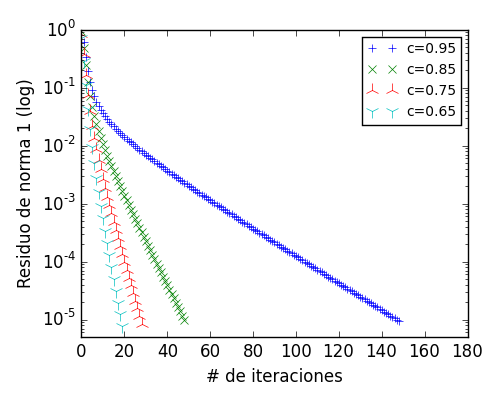
\includegraphics[width=1\textwidth]{imgs/convergencia-stanford.png}
  \caption{\footnotesize{Comparación de la velocidad de convergencia del el método para el dataset web-Stanford.}}
  \label{fig:conv1}
\end{minipage}
\hspace{0.02\textwidth}
\begin{minipage}{0.48\textwidth}
  \centering
    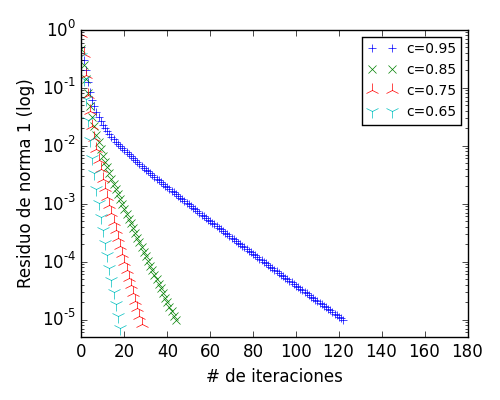
\includegraphics[width=1\textwidth]{imgs/convergencia-notredame.png}
  \caption{\footnotesize{Comparación de la velocidad de convergencia del el método para el dataset web-NotreDame.}}
  \label{fig:conv2}
\end{minipage}
\begin{minipage}{0.5\textwidth}
  \centering
    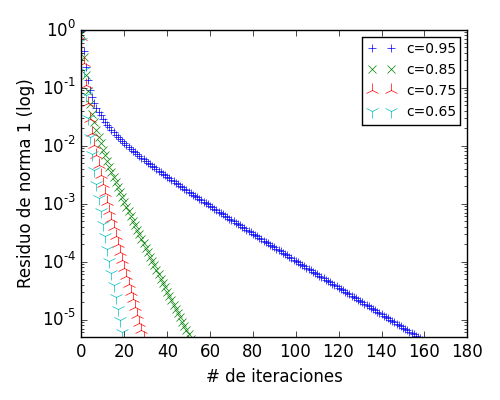
\includegraphics[width=1\textwidth]{imgs/convergencia-google.png}
  \caption{\footnotesize{Comparación de la velocidad de convergencia del el método para el dataset web-Google.}}
  \label{fig:conv3}
\end{minipage}
\end{figure}


Primero notemos algo más o menos sorprendente: la cantidad de iteraciones requeridas por el método no varía demasiado, sobre todo para valores chicos de $c$. Creemos que esto se debe a propiedades generales del método de la potencia, que sin embargo son díficiles de analizar y están fuera del alcance de este trabajo.

Se puede notar además que para los valores más pequeños de $c$ la cantidad de iteraciones correspondientes a cada dataset es prácticamente igual.

Una cosa importante para decir, de la cual vamos a hablar en profundidad más adelante, es que aunque la cantidad de iteraciones sea parecida, el costo de cada iteración es mayor a más grande es la matriz y a más valores no nulos tiene, por lo que las figuras \ref{fig:conv1}, \ref{fig:conv2} y \ref{fig:conv3} no deben intepretarse como el tiempo que requiere el algoritmo para correr.

Sin embargo, una cosa interesante a analizar es qué $c$ usar. Como vimos, usar un $c$ pequeño disminuye el tiempo de cómputo requerido. Sin embargo, disminuir el $c$ también puede impactar en el resultado. Dado que el factor de teletransportación $1-c$ es más alto, de alguna manera el resultado es menos significativo, debido a que se hace más uniforme, como explicamos antes. 
En \cite{Chakrabarti}, por ejemplo, se sugiere que $c$ debería ser elegido basado en la conectividad del grafo.


Otro experimento muy interesante que realizamos es cambiar el criterio de parada del algoritmo iterativo. En particular, lo que hicimos fue cambiar la norma con la que medimos la diferencia entre dos vectores de sucesivas iteraciones. Para ello utilizamos las normas $||-||_1$, $||-||_2$ y $||-||_{\infty}$.

\begin{figure}[H]
\centering

    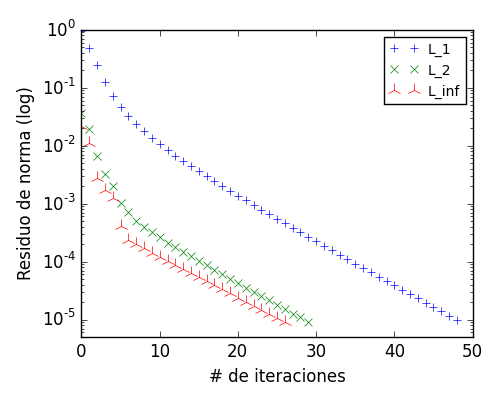
\includegraphics[width=0.6\textwidth]{imgs/convergencia-norma.png}
  \caption{\footnotesize{Comparación de la velocidad de convergencia del el método para el dataset web-Stanford, variando la norma del criterio de parada.}}
  \label{fig:conv-norma}
\end{figure}

Como se observa en la figura \ref{fig:conv-norma}, cuando se utiliza la norma 1 para el criterio de parada, se requieren más iteraciones para terminar. Esto se debe a que la norma 1 es la más \emph{exigente}. 

Se puede probar fácilmente que para todo vector $x$, $||x||_1 \geq ||x||_2 \geq ||x||_{\infty}$ y esto explica claramente los resultados del experimento.



\subsubsection{Rendimiento de PageRank}
A continuación analizaremos el rendimiento del algoritmo de PageRank implementado en este trabajo, es decir, el de \cite{Kamvar2003}. Para ello, utilizaremos los mismos datasets que en la sección anterior.

\begin{figure}[H]
\centering
\begin{tabular}{| c | c | c | c |}
  \hline
  Dataset & Vértices & Aristas & Tiempo (segundos) \\ \hline \hline
  web-Stanford & 281.903 & 2.312.497 & 7.81882 \\ \hline
  web-NotreDame & 325.729 & 1.497.134 & 3.38163 \\ \hline
  web-Google & 916.428 & 5.105.039 & 23.7367 \\ \hline
\end{tabular}

  \caption{\footnotesize{Comparación de los tiempos que requiere el algoritmo para distintos datasets. Fue ejecutado con $c = 0.85$ y $tolerancia = 0.00001$.  Se tomó el promedio de 20 mediciones.}}
  \label{fig:tiempos1}
\end{figure}

Podríamos empezar a sacar conclusiones apresuradas sobre estos datos, pero para que sean más significativos, preferimos realizar otro experimento antes de comenzar el análisis.
Este experimento consiste en dividir el algoritmo en 2: primero el armado de la matriz (recordemos que como representamos la matriz en CRS este no es un paso trivial) y luego el paso de método de la potencia optimizado presentado en \cite{Kamvar2003}.

Esto nos permitirá ver mejor el problema y tener datos más detallados, con el objetivo de poder analizar mejor que es lo que sucede.

\begin{figure}[H]
\centering
\begin{tabular}{| c | c | c | c |}
  \hline
  Dataset & Tiempo total & Armado de matriz & Método de la potencia \\ \hline \hline
  web-Stanford & 7.81882 & 1.8968 & 5.91098 \\ \hline
  web-NotreDame &  3.38163 & 0.978923 & 2.42743 \\ \hline
  web-Google & 23.7367 & 4.30584 & 18.9483 \\ \hline
\end{tabular}

  \caption{\footnotesize{Comparación de los tiempos que requiere el algoritmo para distintos datasets. Fue ejecutado con $c = 0.85$ y $tolerancia = 0.00001$. Se tomó el promedio de 20 mediciones. Todos los tiempos son en segundos. Las sumas probablemente no den bien porque fueron tomadas en diferentes mediciones. }}
  \label{fig:tiempos2}
\end{figure}


Ahora, teniendo toda la información que nos proveen la figura \ref{fig:tiempos1}, \ref{fig:tiempos2} y los experimentos de la sección anterior, podemos hacer un análisis completo y riguroso.

Podemos concluir primero que el paso más costoso del algoritmo es el método de la potencia. Justamente por eso \cite{Kamvar2003} se ocupa de intentar optimizar ese paso, dado que optimizarlo va a impactar fuertemente en el rendimiento general de la aplicación.


Otro aspecto interesante para ver es, como aunque las iteraciones requeridas para cada dataset son bastante similares, el costo de cada operación es muy distinto, pues el tamaño de los vectores varía, y las entradas no nulas de la matriz son distintas. 

De hecho, este experimento nos permite confirmar que el paso más costoso es realizar el producto de la matriz y el vector $P^t x^{(k)}$, ya que se puede ver como el método de la potencia en el caso de web-NotreDame tarda menos que en el caso de web-Stanford, aunque los vectores sean más largos. 

Esto se debe a que la matriz de web-NotreDame es más esparsa, y al multiplicar $Ax$ con $A$ representada en CRS, el costo resulta lineal en la cantidad de elementos no nulos de la matriz. Esta última está intimamente relacionada con la cantidad de aristas del grafo. De esta manera se explica fácilmente el comportamiento a priori extraño de el algoritmo sobre estos datasets.



\newpage
\subsection{PageRank y ligas deportivas}
El conjunto de datos que consideramos para esta sección es el correspondiente al actual torneo de primera división del fútbol argentino. Dicha liga cuenta con las siguientes características relevantes al problema que queremos tratar:
\begin{enumerate}
	\item Hay un total de 30 equipos que juegan todos una vez entre sí. Además, cada equipo juega un partido adicional con su clásico rival.
	\item Los empates son un resultado posible, e incluso muy frecuente. En nuestra implementación de GeM, la posición que tomamos frente a esta situación (que no está contemplada en \cite{Govan2008}) es la de no hacer nada: es decir, si los equipos $i$ y $j$ empataron (o más generalmente, la diferencia absoluta de goles entre todos los partidos que jugaron es 0), entonces en las posiciones $(i,j)$ y $(j,i)$ de nuestra matriz de adyacencia ponemos 0. Consideramos que esta medida es más que razonable, pues en definitiva lo que busca el algoritmo GeM es establecer una \emph{relación de fuerza} entre los equipos a partir de la diferencia de goles que se sacan, la cual, en el caso concreto del empate, es nula. 
	\item El sistema de puntuación estándar es: 3 puntos por partido ganado, 1 por empate y 0 por derrota.
	\item Al momento de realizarse el presente trabajo, sólo se ha jugado hasta la fecha 26 del torneo. Por lo tanto sólo analizaremos los datos hasta la misma. 
\end{enumerate} 

A diferencia de lo que sucedía en la sección (\ref{subsec:pagerank}), aquí no nos interesa realizar un análisis sobre la performance o la convergencia del método, sino más bien un análisis sobre la \emph{calidad} (en algún sentido) de los rankings generados por el mismo, contrastándolos con los reales. Por lo tanto las hipótesis irán en esa dirección. A continuación las enlistamos.

\begin{itemize}
	\item No todos los goles tendrán el mismo peso. Esto es lógico si consideramos la naturaleza del método: si el equipo A le gana al equipo B, que está invicto hasta el momento, por X goles, esto impactará mucho más en el rankeo de A que si le hubiera ganado por X goles a C, un equipo que pierde usualmente. Esto ya plantea una diferencia importante con el método de puntuación estándar, donde en cualquiera de los dos casos A mejoraría su puntaje de la misma manera.

	\item Algo interesante para analizar es la influencia de los empates en los dos tipos de rankeos. Como ya se dijo, un empate en nuestra implementación de GeM no altera la relación de fuerzas entre los equipos. De hecho, a los fines prácticos, un empate es equivalente a que ambos equipos nunca hayan jugado entre sí (en nuestro modelo), por lo que es claro que la matriz de GeM antes o después de un empate es la misma. Sin embargo, con el método estándar los empates sí que modifican el ranking. No alteran la posición relativa de los equipos que empataron, pero claramente puede mejorar la posición de los dos equipos frente al resto (ya que ambos sumaron un punto). Ante esta situación, podemos suponer que los empates van a tener un efecto no despreciable en los resultados reales, siendo una potencial fuente de diferencias con la versión GeM.

	\item Para valores de \emph{c} \footnote{Recordar que 1-\emph{c} era la probabilidad de teletransportación, o en este caso más concretamente, la probabilidad de que un equipo cualquiera pueda ganar contra cualquier otro.} muy chicos los puntajes de los equipos deberían tender a homogeneizarse, generando rankeos poco deseables considerando la \emph{performance} de los equipos. Como contrapartida, para valores de \emph{c} muy altos, el rankeo debería ser más justo.
\end{itemize}


\subsubsection{Análisis cualitativo de los resultados}

\begin{table}[H]
	\center
	\begin{flushright}
	\begin{tabular}{| m{0.405\textwidth} || m{0.385\textwidth} |}
		\rowcolor{LightCyan}
		\hline Método GeM & Método Estándar \\ \hline
	\end{tabular}

	\begin{tabular}{| c | c | c || c | c |}
	  	\hline
	  	\rowcolor{LightCyan}
	  	Posición & Equipo & Puntaje & Equipo & Puntaje \\ \hline \hline
		1 & Boca Juniors & 0.0859387 & Boca Juniors & 58 \\ \hline
		2 & \cellcolor{Gray} Aldosivi & 0.0653494 & San Lorenzo & 54 \\ \hline
		3 & River Plate & 0.063251  & Rosario Central & 52\\ \hline
		4 & San Lorenzo & 0.0624152 & Racing Club & 49\\ \hline
		5 & Rosario Central & 0.048369 & River Plate & 48\\ \hline
		6 & Racing Club & 0.0480862 & Independiente & 45\\ \hline
		7 & San Martín (SJ) & 0.0439307 & Banfield & 43\\ \hline
		8 & Quilmes & 0.0421091 & Belgrano & 43\\ \hline
		9 & Newell's Old Boys & 0.038184 & Tigre & 42\\ \hline
		10 & Vélez Sarsfield & 0.0374806 & Estudiantes (LP) & 42\\ \hline
		11 & Independiente & 0.0363642 & Lanús & 41\\ \hline
		12 & Belgrano & 0.0362427 & Quilmes & 39\\ \hline
		13 & Gimnasia y Esgrima (LP) & 0.0334854 & Unión & 38\\ \hline
		14 & Banfield & 0.0308403 & Gimnasia y Esgrima (LP) & 37\\ \hline
		15 & Estudiantes (LP) & 0.029259 & Newell's Old Boys & 33\\ \hline
		16 & Unión & 0.0287605 & San Martín (SJ) & 32\\ \hline
		17 & Tigre & 0.0272169 & Sarmiento & 30\\ \hline
		18 & Sarmiento & 0.0258276 & \cellcolor{Gray} Aldosivi & 30\\ \hline
		19 & Lanús & 0.0251797 & Temperley & 29\\ \hline
		20 & Huracán & 0.0247069 & Argentinos Juniors & 29\\ \hline
		21 & Defensa y Justicia & 0.0239225 & Olimpo & 29\\ \hline
		22 & Olimpo & 0.0224303 & Defensa y Justicia & 27 \\ \hline
		23 & Arsenal & 0.0208047 & Huracán & 26 \\ \hline
		24 & Godoy Cruz & 0.0174517 & Vélez Sarsfield & 26 \\ \hline
		25 & Temperley & 0.0158447 & Godoy Cruz & 25 \\ \hline
		26 & Crucero del Norte & 0.0156778 & Colón & 24 \\ \hline
		27 & Argentinos Juniors & 0.0153485 & Arsenal & 23 \\ \hline
		28 & Nueva Chicago & 0.0142273 & Atlético de Rafaela & 22 \\ \hline
		29 & Atlético de Rafaela & 0.0112011 & Nueva Chicago & 17 \\ \hline
		30 & Colón & 0.010094 & Crucero del Norte & 14 \\ \hline
	\end{tabular}
	\end{flushright}
	\caption{\footnotesize Ranking correspondiente a la fecha 26 usando el método GeM, para un valor de $c = 0.85$, y el método estándar.}
	\label{tab:fecha26}
\end{table}

Al observar la tabla \ref{tab:fecha26}, notamos como primera gran sorpresa que Aldosivi (8 ganados-12 perdidos) aparece segundo en nuestro ranking GeM, siendo que en la realidad ocupa la posición 18. Este resultado, \emph{a priori} extraño, parece cobrar sentido si consideramos lo sucedido en la fecha 13 del torneo: Aldosivi goleó por 3-0 a Boca, el actual puntero según nuestro ranking (y también según el ranking oficial). En efecto, si vemos la tabla \ref{tab:fecha12-13} podemos apreciar como la contundente derrota de Boca (que hasta ese momento estaba primero) permitió catapultar a Aldosivi del cuarto al primer puesto, con una diferencia respecto del segundo particularmente amplia. 

Vale destacar, que en la realidad, este resultado tuvo un impacto significativamente menor: Boca siguió estando primero, con la pequeña diferencia de que fue alcanzado por San Lorenzo, mientras que Aldosivi se mantuvo lejos de la punta, en el puesto 8.

En los sucesivos partidos, Aldosivi sufrió una larga lista de derrotas, sin embargo, como vimos en la tabla \ref{tab:fecha26} esto apenas si perjudicó su posición. Podemos decir que esto es producto del \emph{batacazo} que dió frente a Boca, que mantuvo durante casi la totalidad del torneo su hegemonía por sobre los otros equipos. Dicho de otra forma, la suerte de Aldosivi quedó en algún punto supeditada a la de Boca, pues entre mejor le fuera a este último, más significativos serían los 3 goles que le había hecho para su propio puntaje. Esto sucede a tal punto que, a la fecha siguiente, Boca pierde 2-0 con Velez pero en lugar de perjudicarlo genera que, posiblemente en combinación con el hecho de que Aldosivi también perdiera por una diferencia de un gol, y de que River (quien había perdido el superclásico) ganara por 2, vuelva a estar puntero, desplazando a Aldosivi al tercer puesto. Es decir que lo importante para rescatar de este úlimo hecho, es que que al finalizar la fecha 14 los 3 goles de Aldosivi ante Boca perdían un poco de peso, pues ahora, en total, este tenía 2 goles más en su contra.

Luego, por todo lo dicho hasta aquí, creemos que nuestra primer hipótesis, concerniente a la distinta importancia que se le asigna a los goles según la performance del equipo que los recibe, queda verificada.  

\begin{table}[H]
	\center
	\begin{flushright}
	\begin{tabular}{| m{16.65em} || m{17.15em} |}
		\rowcolor{LightCyan}
		\hline Fecha 12 & Fecha 13 \\ \hline
	\end{tabular}

	\begin{tabular}{| c | c | c || c | c |}
	  	\hline
	  	\rowcolor{LightCyan}
	  	Posición & Equipo & Puntaje & Equipo & Puntaje \\ \hline \hline
		1 & \cellcolor{Gray} Boca Juniors & 0.108944 &  \cellcolor{Gray} Aldosivi & 0.117217 \\ \hline
		2 & River Plate & 0.0815019 & \cellcolor{Gray} Boca Juniors & 0.0892615 \\ \hline
		3 & Rosario Central & 0.0735106 & River Plate & 0.0657072 \\ \hline
		4 & \cellcolor{Gray} Aldosivi & 0.0546487 & Rosario Central & 0.0608375 \\ \hline
		5 & San Lorenzo & 0.0511854 & Banfield & 0.0546665 \\ \hline
		6 & Racing Club & 0.046461 & San Lorenzo & 0.0497559 \\ \hline
		7 & Belgrano & 0.0464054 & Gimnasia y Esgrima (LP) & 0.0478387 \\ \hline
		8 & Banfield & 0.0440866 & Vélez Sarsfield & 0.0426006 \\ \hline
		9 & San Martín (SJ) & 0.0433587 & Racing Club & 0.0418281\\ \hline
		10 & Newell's Old Boys & 0.0353829 & Newell's Old Boys & 0.036451 \\ \hline
		11 & Lanús & 0.0320765 & Belgrano & 0.0356502 \\ \hline
		12 & Gimnasia y Esgrima (LP) & 0.029684 & San Martín (SJ) & 0.0350081 \\ \hline
		13 & Sarmiento & 0.0263866 & Lanús & 0.0346346 \\ \hline
		14 & Arsenal & 0.0252073 & Estudiantes (LP) & 0.025968 \\ \hline
		15 & Huracán & 0.0241481 & Argentinos Juniors & 0.0241652 \\ \hline
		16 & Estudiantes (LP) & 0.024007 & Huracán & 0.0215508 \\ \hline
		17 & Tigre & 0.023322 & Godoy Cruz & 0.0211769 \\ \hline
		18 & Vélez Sarsfield & 0.0229058 & Sarmiento & 0.0210192 \\ \hline
		19 & Independiente & 0.0224838 & Arsenal & 0.0200022 \\ \hline
		20 & Argentinos Juniors & 0.0221471 & Unión & 0.0199389 \\ \hline
		21 & Temperley & 0.0212702 & Defensa y Justicia & 0.019309 \\ \hline
		22 & Unión & 0.0212572 & Tigre & 0.0179675 \\ \hline
		23 & Defensa y Justicia & 0.0206203 & Independiente & 0.0170322 \\ \hline
		24 & Quilmes & 0.0168138 & Temperley & 0.0158759 \\ \hline
		25 & Godoy Cruz & 0.0166558 & Quilmes & 0.0158634 \\ \hline
		26 & Colón & 0.0159257 & Crucero del Norte & 0.0127548 \\ \hline
		27 & Olimpo & 0.0135905 & Colón & 0.0106429 \\ \hline
		28 & Atlético de Rafaela & 0.0130908 & Olimpo & 0.00977677 \\ \hline
		29 & Crucero del Norte & 0.0127524 & Atlético de Rafaela & 0.00877535 \\ \hline
		30 & Nueva Chicago & 0.0101696 & Nueva Chicago & 0.00672374 \\ \hline
	\end{tabular}
	\end{flushright}
	\caption{\footnotesize Posiciones de las fechas 12 y 13 calculadas con GeM y $c = 0.85$.}
	\label{tab:fecha12-13}
\end{table}

A continuación veamos, con un experimento muy simple pero ilustrativo, como el tomar un modelo que ignora los empates frente a otro que les da cierta importancia puede afectar sensiblemente la tabla de posiciones. Para eso veamos que sucede al considerar los resultados de la primera fecha que se muestran en la tabla \ref{tab:fecha1}. Rápidamente, podemos notar que en ambos casos los equipos que comparten el primer lugar son los mismos: los que ganaron su respectivo partido. Sin embargo, en la versión GeM tanto los equipos que empataron como los que perdieron tienen todos la última posición, cosa que no ocurre en el modelo estándar, donde los equipos que empataron están segundos mientras que los que perdieron están últimos. Esto en principio parece un rankeo un poco injusto para los que empataron, que son puestos al mismo nivel de los perdedores.

Vale decir que esta es una situación muy particular: al ser la primer fecha, la matriz de adyacencias no solo será muy esparsa, sino que al menos la mitad de sus filas serán 0 (correspondientes a los equipos que ganaron o empataron)mientras que de la otra mitad a lo sumo tendrán un coeficiente no nulo (correspondientes a los equipos que perdieron). Debido a esto, es que, por ejemplo, todos los equipos que ganaron tienen el mismo puntaje a pesar de que hayan ganado por distintas diferencias (donde la más grande fue de River por 3 goles). Por lo tanto, este debe considerarse como un ejemplo particular donde el dar puntos a los empates genera una situación un poco más justa, pero no debe extrapolarse una conclusión apresurada y afirmar que esto valga para cualquier caso. La experimentación necesaria, así como el análisis que se requiere, para determinar esas conclusiones son de una dificultad no trivial (especialmente considerando que en el caso de GeM el puntaje de un equipo no depende sólo de sus resultados sino también de los de sus adversarios), por lo que no lo abordaremos en más profundidad en este trabajo.

\begin{table}[H]
	\center
	\begin{flushright}
	\begin{tabular}{| m{0.405\textwidth} || m{0.3925\textwidth} |}
		\rowcolor{LightCyan}
		\hline Método GeM & Método Estándar \\ \hline
	\end{tabular}

	\begin{tabular}{| c | c | c || c | c |}
	  	\hline
	  	\rowcolor{LightCyan}
	  	Posición & Equipo & Puntaje & Equipo & Puntaje \\ \hline \hline
		1 & \cellcolor{green!20}River Plate & 0.0450669 & \cellcolor{green!20}Lanús & 3 \\ \hline
		2 & \cellcolor{green!20}Lanús & 0.0450669 & \cellcolor{green!20}Vélez Sarsfield & 3 \\ \hline 
		3 & \cellcolor{green!20}Vélez Sarsfield & 0.0450669 & \cellcolor{green!20}Unión & 3 \\ \hline 
		4 & \cellcolor{green!20}Temperley & 0.0450669 & \cellcolor{green!20}Temperley & 3 \\ \hline 
		5 & \cellcolor{green!20}Rosario Central & 0.0450669 & \cellcolor{green!20}San Lorenzo & 3 \\ \hline 
		6 & \cellcolor{green!20}Independiente & 0.0450669 & \cellcolor{green!20}Rosario Central & 3 \\ \hline 
		7 & \cellcolor{green!20}Estudiantes (LP) & 0.0450669 & \cellcolor{green!20}River Plate & 3 \\ \hline 
		8 & \cellcolor{green!20}Argentinos Juniors & 0.0450669 & \cellcolor{green!20}Independiente & 3 \\ \hline 
		9 & \cellcolor{green!20}Boca Juniors & 0.0450669 & \cellcolor{green!20}Estudiantes (LP) & 3 \\ \hline 
		10 & \cellcolor{green!20}Belgrano & 0.0450669 & \cellcolor{green!20}Defensa y Justicia & 3 \\ \hline 
		11 & \cellcolor{green!20}Defensa y Justicia & 0.0450669 & \cellcolor{green!20}Argentinos Juniors & 3 \\ \hline 
		12 & \cellcolor{green!20}Unión & 0.0450669 & \cellcolor{green!20}Belgrano & 3 \\ \hline 
		13 & \cellcolor{green!20}San Lorenzo & 0.0450669 & \cellcolor{green!20}Boca Juniors & 3 \\ \hline
		14 & \cellcolor{yellow!20}Olimpo & 0.0243606 & \cellcolor{yellow!20}Crucero del Norte & 1 \\ \hline
		15 & \cellcolor{yellow!20}Tigre & 0.0243606 & \cellcolor{yellow!20}Tigre & 1 \\ \hline
		16 & \cellcolor{yellow!20}Arsenal & 0.0243606 & \cellcolor{yellow!20}San Martín (SJ) & 1 \\ \hline
		17 & \cellcolor{yellow!20}Sarmiento & 0.0243606 & \cellcolor{yellow!20}Godoy Cruz & 1 \\ \hline
		18 & \cellcolor{yellow!20}San Martín (SJ) & 0.0243606 & \cellcolor{red!20}Newell's Old Boys & 0 \\ \hline
		19 & \cellcolor{yellow!20}Atlético de Rafaela & 0.0243606 & \cellcolor{red!20}Nueva Chicago & 0 \\ \hline
		20 & \cellcolor{yellow!20}Banfield & 0.0243606 & \cellcolor{red!20}Olimpo & 0 \\ \hline
		21 & \cellcolor{yellow!20}Racing Club & 0.0243606 &\cellcolor{red!20} Quilmes & 0 \\ \hline
		22 & \cellcolor{yellow!20}Quilmes & 0.0243606 &\cellcolor{red!20} Racing Club & 0 \\ \hline
		23 & \cellcolor{yellow!20}Colón & 0.0243606 & \cellcolor{red!20}Aldosivi & 0 \\ \hline
		24 & \cellcolor{yellow!20}Nueva Chicago & 0.0243606 & \cellcolor{red!20}Colón & 0 \\ \hline
		25 & \cellcolor{yellow!20}Newell's Old Boys & 0.0243606 & \cellcolor{red!20}Banfield & 0 \\ \hline
		26 & \cellcolor{yellow!20}Aldosivi & 0.0243606 & \cellcolor{red!20}Huracán & 0 \\ \hline
		27 & \cellcolor{yellow!20}Huracán & 0.0243606 & \cellcolor{red!20}Sarmiento & 0 \\ \hline
		28 & \cellcolor{yellow!20}Godoy Cruz & 0.0243606 & \cellcolor{red!20}Atlético de Rafaela & 0 \\ \hline
		29 & \cellcolor{yellow!20}Gimnasia y Esgrima (LP) & 0.0243606  & \cellcolor{red!20}Arsenal & 0 \\ \hline
		30 & \cellcolor{yellow!20}Crucero del Norte & 0.0243606 &\cellcolor{red!20} Gimnasia y Esgrima (LP) & 0 \\ \hline
	\end{tabular}
	\end{flushright}
	\caption{\footnotesize Ranking correspondiente a la fecha 1 usando el método GeM, para un valor de  $c = 0.85$, y el método estándar. Los sombreados verde, amarillo y rojo señalan la posición del equipo que puede ser 1º, 2º o 3º respectivamente.}
	\label{tab:fecha1}
\end{table}

Finalmente, analicemos el efecto de variar el valor del $c$. Para esto consideremos los resultados expuestos en la tabla \ref{tab:variosc}, que nos muestra el rankeo correspondiente a la fecha 26 usando GeM con dos valores extremos de $c$: $0.1$ y $0.99$. Recordar que el primero es el caso en que la probabilidad de que un equipo pierda contra otro depende mucho menos de los resultados previos y tiende a ser la misma para todos, mientras que el segundo es el opuesto: los resultados previos determinan casi totalmente la probabilidad de que un equipo pierda con otro.

Curiosamente vemos que no hay diferencias grandes entre ambos rankings. De hecho en muchos casos, la posición del equipo no cambió. Aunque en efecto, como habíamos supuesto, el $c$ pequeño hizo que las puntuaciones se homogeneizaran, vemos que en la práctica la ventaja que le da a un equipo ser más goleador que otros y ganarle a equipos importantes sigue siendo lo suficientemente significativa como para que el ranking no presente resultados absurdos (como que un equipo que rankeaba de la mitad para abajo de la tabla con un $c$ alto, pase a estar en los primeros lugares con uno bajo). De hecho, más bien pareciera que pasa lo contrario. 

Si volvemos a considerar el particular caso de Aldosivi, vemos que al tomar un $c$ más cercano a 0 su posición en la tabla empeoró en cuatro posiciones (respecto de las versiones con $c=0.85$ $c=0.99$). Esto es muy razonable si tenemos en cuenta que el buen rankeo de Aldosivi estaba fuertemente basado en un resultado aislado (un \emph{outlier} si se quiere) como fue su amplia victoria sobre Boca, el equipo que mejor $performance$ tuvo en el campeonato. No sólo eso, sino que también le gano por 1-0 a San Lorenzo, otro de los principales equipos. Al reducir la incidencia de los resultados de todos los partidos sobre el cálculo de los puntajes, Aldosivi recibe muchos menos ``votos'' de Boca o San Lorenzo, pues los mismos ahora se reparten más equitativamente entre todos los equipos, y como Aldosivi tuvo pocas victorias en general se ve perjudicado con este cambio.

De la misma forma, pasa algo muy parecido con Vélez (el equipo que más posiciones bajó al considerar el $c$ más chico) que también le ganó a Boca (2-0) y al mismo Aldosivi (2-0), pero en términos generales apenas pudo ganar 6 partidos y perdió 13.

De hecho, la tendencia general es que la subtabla correspondiente a $c=0.1$ tiende a asemejarse mucho más al ranking oficial, que puede verse en la tabla \ref{tab:fecha26}, de que lo hace la subtabla correspondiente a $c=0.99$. Recordar que el método estándar no considera las diferencias de goles, y sí considera la cantidad de victorias, derrotas y empates. Podemos pensar entonces, basándonos en lo que venimos viendo, que un valor más chico de $c$ genera que la cantidad de victorias pese más y al mismo tiempo reduce la importancia de goleadas muy abultadas, lo cual puede ser útil para reducir el impacto de resultados aislados como el de Aldosivi o el de Velez.

En resumen, llegamos a la conclusión de que, contra lo que habíamos supuesto en las hipótesis, la utilización de un $c$ bajo puede dar resultados más sensatos que la de uno muy alto, pues evita que equipos que muestran un bajo rendimiento logren un excelente rankeo sólo por \emph{batacazos} aislados. Por el contrario, el $c$ demasiado alto acrecenta estas diferencias. Particularmente, encontramos que, al menos para este caso, un valor de $c=0.35$ resultado bastante apropiado, basándonos en que, en sentido decreciente, es el primer valor para el cual Aldosivi pasa a estar por debajo de Racing (14 ganados-5 perdidos), que mostró un mejor nivel a lo largo del torneo. No ponemos el ranking obtenido para este valor dado que no aporta nada nuevo a la discución.

\begin{table}[H]
	\center
	\begin{flushright}
	\begin{tabular}{| m{0.405\textwidth} || m{0.416\textwidth} |}
		\rowcolor{LightCyan}
		\hline $c=0.1$ & $c=0.99$ \\ \hline
	\end{tabular}

	\begin{tabular}{| c | c | c || c | c |}
	  	\hline
	  	\rowcolor{LightCyan}
	  	Posición & Equipo & Puntaje & Equipo & Puntaje \\ \hline \hline
		1 & Boca Juniors & 0.0391469 & Boca Juniors & 0.0945905 \\ \hline
		2 & San Lorenzo & 0.0370791 & \cellcolor{green!20}Aldosivi & 0.0744865 \\ \hline
		3 & River Plate & 0.0368742 & River Plate & 0.0675502 \\ \hline
		4 & Racing Club & 0.0357606 & San Lorenzo & 0.0656075 \\ \hline
		5 & Rosario Central & 0.0353159 & Rosario Central & 0.0505593 \\ \hline
		6 & \cellcolor{green!20}Aldosivi & 0.0347251 & Racing Club & 0.049052 \\ \hline
		7 & Quilmes & 0.0344085 & San Martín (SJ) & 0.0468815 \\ \hline
		8 & Independiente & 0.0341835 & Quilmes & 0.0433725 \\ \hline
		9 & Belgrano & 0.034173 & \cellcolor{blue!20}Vélez Sarsfield & 0.0410949 \\ \hline
		10 & San Martín (SJ) & 0.033846 & Newell's Old Boys & 0.039274 \\ \hline
		11 & Newell's Old Boys & 0.0337048 & Independiente & 0.0355528 \\ \hline
		12 & Gimnasia y Esgrima (LP) & 0.033465 & Belgrano & 0.0354938 \\ \hline
		13 & Lanús & 0.0334376 & Gimnasia y Esgrima (LP) & 0.0337113 \\ \hline
		14 & Banfield & 0.0332383  & Banfield & 0.0304023 \\ \hline
		15 & Tigre & 0.0331063 & Estudiantes (LP) & 0.0290798 \\ \hline
		16 & Estudiantes (LP) & 0.0326988 & Unión & 0.0283743 \\ \hline
		17 & Unión & 0.0325988 & Tigre & 0.0260657 \\ \hline
		18 & Sarmiento & 0.0325042 & Sarmiento & 0.0245763 \\ \hline
		19 & \cellcolor{blue!20}Vélez Sarsfield & 0.0324059 & Defensa y Justicia & 0.023483 \\ \hline
		20 & Arsenal & 0.0322979 & Huracán & 0.0229007 \\ \hline
		21 & Huracán & 0.0322357 & Lanús & 0.0220692 \\ \hline
		22 & Defensa y Justicia & 0.0318777 & Olimpo & 0.0215218 \\ \hline
		23 & Olimpo & 0.0318753 & Arsenal & 0.0179464 \\ \hline
		24 & Argentinos Juniors & 0.0317518 & Godoy Cruz & 0.0142913 \\ \hline
		25 & Godoy Cruz & 0.0317468 & Crucero del Norte & 0.012915 \\ \hline
		26 & Temperley & 0.0315835 & Temperley & 0.0124947 \\ \hline
		27 & Crucero del Norte & 0.0313297 & Argentinos Juniors & 0.0115357 \\ \hline
		28 & Nueva Chicago & 0.0310144 & Nueva Chicago & 0.0114375 \\ \hline
		29 & Atlético de Rafaela & 0.0308366 & Atlético de Rafaela & 0.00759916 \\ \hline
		30 & Colón & 0.0307777 & Colón & 0.00608033 \\ \hline
	\end{tabular}
	\end{flushright}
	\caption{\footnotesize Ranking correspondiente a la fecha 26 usando el método GeM para dos valores de $c$ distintos: $0.1$ y $0.99$}
	\label{tab:variosc}
\end{table}

\newpage

\section{Conclusiones}
A continuación pasamos en limpio las conclusiones a las que llegamos con la realización del presente trabajo práctico.

Con respecto al método pagerank:
\begin{itemize}
	\item En lo concerniente a la convergerncia del método concluimos que:
		\begin{itemize}
			\item Para un mismo valor de $c$, la cantidad de iteraciones requeridas para distintos datasets varía poco, especialmente si $c$ es chico. Si $c$ es muy cercano a 1, entonces la cantidad de iteraciones es menor para grafos más disconexos.
			\item Entre más chico sea el valor de $c$, más rápido va a converger pagerank. Sin embargo, esto también produce que el resultado sea menos significativo, por lo cual es importante tener un buen criterio para la elección del $c$, por ejemplo, considerando la conectividaad del grafo.
			\item Al modificar la norma que usamos para determinar el criterio de parada, vemos que usar una norma $p$ disminuye la cantidad de iteraciones cuanto mayor es $p$, pero al mismo tiempo genera que el resultado sea menos preciso. De forma similar, un $p$ más chico produce el efecto contrario.
		\end{itemize}
	\item Sobre la performance del método, vimos que el paso más costoso del algoritmo es realizar el método de la potencia. Pese a que la cantidad de iteraciones para dos datasets distintos fuera prácticamente igual, el tiempo de cómputo efectivo era distinto pues el costo de realizar cada producto de matriz por vector dependía linealmente de la cantidad de coeficientes no nulos de la matriz (debido a la representación CRS utilizada para la misma). Por lo tanto, para matrices más esparsas (correspondientes a grafos más disconexos), se requiere menos tiempo de cómputo.
	\item En lo respectivo al análisis cualitativo, concluimos que pagerank permite conseguir rankings más realistas que In-Deg, como resultado de considerar no solo la cantidad de enlaces entrantes sino también la importancia relativa de los mismos. Además, vimos que pagerank le permite a cada página mejorar parcialmente su posición al agregar un mayor número de enlaces salientes. Como trabajo a futuro se plantea el generalizar y profundizar las propiedades vistas. 
\end{itemize}

Con respecto al modelo GeM:
\begin{itemize}
	\item Vimos que el método propuesto por Govan et al. no es \emph{democrático}, en el sentido de que tiene mucha más relevancia sacarle un diferencia positiva a un equipo que está bien rankeado que a uno que no lo está. Esta es una clara diferencia  con el método tradicional de rankeo del fútbol, en la cual ganarle a cualquier equipo da la misma cantidad de puntos. Así mismo, las diferencias grandes de marcador son un factor clave pues favorecen más al vencedor, cosa que no se da con el método clásico.
	\item En la misma línea de lo anterior, vimos que el valor de $c$ afecta de forma directa la calidad del rankeo: si bien en términos generales puede no producir grandes cambios, el tomar un valor muy cercano a 1 genera que equipos de un bajo rendimiento general puedan aprovecharse demasiado de una victoria aislada a algún equipo bien posicionado. Mientras tanto, tomar un valor más cercano a 0 amortigua este efecto, dándole mayor importancia a la cantidad de partidos ganados. Particularmente, llegamos a la conclusión de que un valor para $c$ cercano a $0.35$ genera rankings sensatos (al menos para el caso de una liga de las características mencionadas en la sección (\ref{subsec:ligas})), logrando entonces un buen promedio entre la importancia de vencer a equipos importantes, así como marcar diferencias amplias de goles, y tener un \emph{ratio} razonablemente bueno de victorias/derrotas. Esto es especialmente importante en el caso del fútbol donde, a diferencia de otros deportes como el rugby o el tennis, no es raro que se produzcan resultados sorpresivos.  
	\item Por otro lado, encontramos que el no considerar los empates con el método GeM puede traer disparidades. Sin embargo, un análisis más profundo sobre este aspecto queda pendiente para trabajos posteriores, así como la realización de variaciones del método que manejen el caso de los empates de forma distinta. Algunas ideas en este sentido podrían ser poner en la posición $(i,j)$ y $(j,i)$ de la matriz de adyacencias la cantidad de goles por la que empataron los equipos $i$ y $j$, o bien, siempre poner 1. También queda en el tintero probar la versión generalizada del modelo GeM que se propone al final de \cite{Govan2008}, con la cual se podrían considerar otras estadísticas como posesión del balón, cantidad de tarjetas, etc.
\end{itemize}
\newpage

\section{Apéndices}
\subsection{Proposiciones}

\subsubsection{Proposición 1}
\label{subsub:prop1}
Si $P \in R^{n\times n}$ es una matriz de transición, es decir $0 \leq P_{ij} \leq 1$, y $\sum_j P_{ij} = 1 \ \forall i\in\{1,...,n\}$, entonces el mayor autovalor en módulo de $P^t$ es 1, y en particular tiene a 1 como autovalor (eventualmente podría tener tamién a -1).

\textbf{Demostración} Primero veamos que si $\lambda$ es autovalor de $P^t$, entonces $|\lambda| \leq 1$.

Vale que $\rho(P^t) \leq ||P^t||$, $\rho(P^t)$ el radio espectral y $||-||$ cualquier norma inducida. En particular, si tomamos la norma 1, $||P^t||_1 = 1$, pues todas las columnas suman 1, pues $P$ es de transición. Entonces $|\lambda| \leq \rho(P^t) \leq 1$.

Ahora, como las filas de $P$ suman 1, si multiplico $P (1, ..., 1)^t = (1, ..., 1)^t$. Es decir que 1 es autovalor de $P$. Entonces, como $P$ y $P^t$ tienen los mismos autovalores, 1 es autovalor de $P^t$, que es lo que queríamos ver.

\textbf{Observación} Probamos que 1 es efectivamente autovalor de la matriz, pero nada nos garantiza que -1 no lo sea. Sin embargo, si al aplicar el método de la potencia empezamos con un vector de todas entradas positivas (como lo hacemos), el resultado final también tendrá todas entradas positivas, resultando en un autovector asociado a autovalor 1.



\newpage
% si se descomenta esto, aparecen todas las cosas de la bibliografia, hasta
% las que nunca fueron citadas en el TP. es una eleccion de diseño.
% \nocite{*}
\printbibliography



\end{document}
